\chapter{Análisis para $Q = \num{0.75}$}
\label{chap:q075}

\section{Función de transferencia}

Con $R = \qty{100}{\ohm}$, $L = \qty{28.23}{\milli\henry}$ y $C = \qty{5.02}{\micro\farad}$, los
coeficientes de la ecuación~\eqref{eq:tf-componentes} resultan

\begin{gather*}
  \frac{R}{L} = \frac{\qty{100}{\ohm}}{\qty{28.23}{\milli\henry}} = \num{3542.33}, \qquad
  \frac{1}{LC} = \frac{1}{\qty{28.23}{\milli\henry} \cdot \qty{5.02}{\micro\farad}} = \num{7056436},
\end{gather*}

y la función de transferencia del filtro es

\begin{equation}
  H_2(s) = \frac{s^2}{s^2 + \num{3542.33}\, s + \num{7056436}}
         = \frac{s^2}{\left(s + \num{1771.17} + j\,\num{1979.75}\right)
                       \left(s + \num{1771.17} - j\,\num{1979.75}\right)}.
  \label{eq:tf-q075}
\end{equation}

\section{Raíces y lugar de raíces}

En este caso el discriminante del polinomio característico es negativo
($\num{3542.33}^2 - 4 \cdot \num{7056436} < 0$) y las raíces son complejas conjugadas:

\begin{gather*}
  s_{1,2} = -\sigma \pm j\,\omega_d = \num{-1771.17} \pm j\,\num{1979.75}\ \unit{\radian\per\second},
\end{gather*}

con parte real $\sigma = \xi\omega_0 = \num{1771.17}$ y pulsación amortiguada
$\omega_d = \omega_0\sqrt{1 - \xi^2} = \num{1979.75}$. Junto con el cero doble en el origen, su ubicación
se muestra en la Figura~\ref{fig:polos-q075}. Los polos se encuentran sobre una circunferencia de radio
$\omega_0 = \qty{2656.4}{\radian\per\second}$ y forman con el semieje real negativo un ángulo
$\theta = \arccos\xi = \qty{48.2}{\degree}$.

\begin{figure}[!ht]
  \centering
  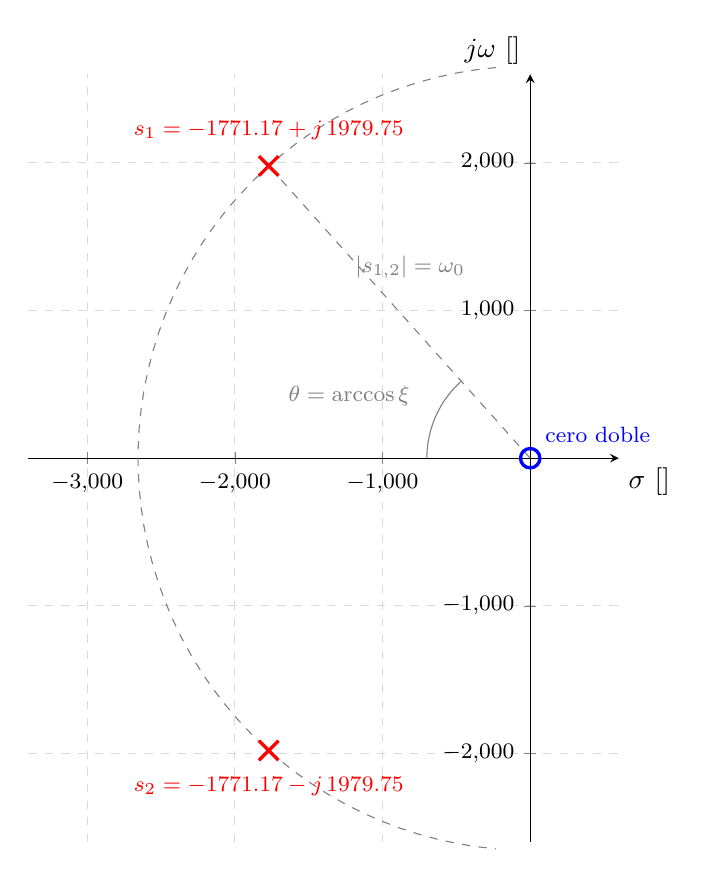
\begin{tikzpicture}
  \begin{axis}[
    % escala igual en ambos ejes: 4000 x 5200 rad/s sobre 7,5 cm x 9,75 cm
    scale only axis, width=7.5cm, height=9.75cm,
    axis lines=middle,
    xlabel={$\sigma$ [\unit{\radian\per\second}]},
    ylabel={$j\omega$ [\unit{\radian\per\second}]},
    xlabel style={at={(ticklabel* cs:1)}, anchor=north west},
    ylabel style={at={(ticklabel* cs:1)}, anchor=south east},
    xmin=-3400, xmax=600, ymin=-2600, ymax=2600,
    xtick={-3000,-2000,-1000},
    ytick={-2000,-1000,1000,2000},
    grid=both, grid style={gray!30, dashed},
    tick label style={font=\footnotesize},
    clip=false,
  ]
    % circunferencia de radio omega_0 sobre la que se ubican los polos
    \addplot[domain=95:265, samples=60, dashed, gray, no marks] ({2656.4*cos(x)}, {2656.4*sin(x)});
    \addplot[dashed, gray, no marks] coordinates {(0,0) (-1771.17,1979.75)};
    \addplot[domain=131.8:180, samples=20, gray, no marks] ({700*cos(x)}, {700*sin(x)});
    \addplot[only marks, mark=x, mark size=5pt, very thick, red]
      coordinates {(-1771.17,1979.75) (-1771.17,-1979.75)};
    \addplot[only marks, mark=o, mark size=3.5pt, very thick, blue] coordinates {(0,0)};
    \node[above=6pt, red, font=\footnotesize] at (axis cs:-1771.17,1979.75)
      {$s_1 = \num{-1771.17} + j\,\num{1979.75}$};
    \node[below=6pt, red, font=\footnotesize] at (axis cs:-1771.17,-1979.75)
      {$s_2 = \num{-1771.17} - j\,\num{1979.75}$};
    \node[above right=2pt, blue, font=\footnotesize] at (axis cs:0,0) {cero doble};
    \node[gray, font=\footnotesize, anchor=south west] at (axis cs:-1250,1150) {$|s_{1,2}| = \omega_0$};
    \node[gray, font=\footnotesize, anchor=east] at (axis cs:-750,420) {$\theta = \arccos\xi$};
  \end{axis}
\end{tikzpicture}

  \caption{Ubicación de polos y ceros de $H_2(s)$ en el plano complejo.}
  \label{fig:polos-q075}
\end{figure}

\section{Factor de amortiguamiento}

De la ecuación~\eqref{eq:xi},

\begin{equation}
  \xi = \frac{1}{2Q} = \frac{1}{2 \cdot \num{0.75}} = \num{0.667},
  \label{eq:xi-q075}
\end{equation}

valor menor que la unidad, en concordancia con el par de raíces complejas conjugadas. La constante de
corrección vale $K = \num{1.0570}$, es decir, la pulsación natural
$\omega_0 = \qty{2656.5}{\radian\per\second}$ queda apenas por encima de la pulsación de corte
($\qty{2513.3}{\radian\per\second}$).

\section{Respuesta temporal}

Ante un escalón unitario, $V_i(s) = 1/s$, la salida en el dominio de Laplace es

\begin{equation}
  V_o(s) = H_2(s)\, V_i(s)
         = \frac{s}{\left(s + \num{1771.17}\right)^2 + \num{1979.75}^2}.
  \label{eq:vo-q075}
\end{equation}

Para antitransformar se suma y resta $\sigma$ en el numerador, de modo de expresar la función como
combinación de las transformadas de $e^{-\sigma t}\cos(\omega_d t)$ y $e^{-\sigma t}\sin(\omega_d t)$:

\begin{gather*}
  V_o(s) = \frac{s + \num{1771.17}}{\left(s + \num{1771.17}\right)^2 + \num{1979.75}^2}
         - \frac{\num{1771.17}}{\num{1979.75}} \cdot
           \frac{\num{1979.75}}{\left(s + \num{1771.17}\right)^2 + \num{1979.75}^2}, \\[4pt]
  \frac{\sigma}{\omega_d} = \frac{\num{1771.17}}{\num{1979.75}} = \num{0.8946}.
\end{gather*}

La respuesta temporal resulta entonces

\begin{equation}
  v_o(t) = e^{-\num{1771.17}\, t}
           \left[\cos\left(\num{1979.75}\, t\right) - \num{0.8946}\, \sin\left(\num{1979.75}\, t\right)\right] u(t),
  \label{eq:vo-t-q075}
\end{equation}


La Figura~\ref{fig:escalon-q075} muestra la respuesta junto con
su envolvente exponencial. Nuevamente $v_o(0^+) = 1$, pero ahora la salida cruza por cero, alcanza un
subpico apreciable y oscila con pulsación $\omega_d$ dentro de la envolvente
$\pm\frac{\omega_0}{\omega_d} e^{-\sigma t}$ hasta extinguirse.

\begin{figure}[!ht]
  \centering
  \begin{tikzpicture}
  \begin{axis}[
    width=0.9\textwidth, height=0.5\textwidth,
    xlabel={$t$ [\unit{\milli\second}]}, ylabel={Tensión [\unit{\volt}]},
    xmin=0, xmax=4, ymin=-0.35, ymax=1.1,
    grid=both, grid style={gray!30, dashed},
    legend pos=north east, legend cell align=left, legend style={font=\footnotesize},
    tick label style={font=\footnotesize},
    samples=400, domain=0:4, no marks,
  ]
    \addplot[gray, thick, dotted] {1};
    \addlegendentry{$v_i(t)$ (escalón unitario)}
    \addplot[blue, very thick]
      {exp(-1.77117*x)*(cos(deg(1.97975*x)) - 0.8946*sin(deg(1.97975*x)))};
    \addlegendentry{$v_o(t)$ para $Q = \num{0.75}$}
    \addplot[orange, dashed, thick] {1.3416*exp(-1.77117*x)};
    \addlegendentry{envolvente $\pm\frac{\omega_0}{\omega_d}e^{-\sigma t}$}
    \addplot[orange, dashed, thick, forget plot] {-1.3416*exp(-1.77117*x)};
    \addplot[red, dashed] {0.02};
    \addlegendentry{banda de $\pm\qty{2}{\percent}$}
    \addplot[red, dashed, forget plot] {-0.02};
    \addplot[only marks, mark=*, mark size=1.8pt, black, forget plot] coordinates {(0.850,-0.222)};
    \node[below right=2pt, font=\footnotesize] at (axis cs:0.850,-0.222)
      {subpico \qty{-22.2}{\percent} en $t = \qty{0.85}{\milli\second}$};
    \addplot[only marks, mark=*, mark size=1.8pt, black, forget plot] coordinates {(0.425,0)};
    \node[above right=2pt, font=\footnotesize] at (axis cs:0.425,0) {$t = \qty{0.425}{\milli\second}$};
    \draw[dashed, gray] (axis cs:1.82,-0.35) -- (axis cs:1.82,0.5)
      node[pos=1, above, font=\footnotesize, black] {$t_s = \qty{1.82}{\milli\second}$};
  \end{axis}
\end{tikzpicture}

  \caption{Respuesta al escalón unitario del filtro con $Q = \num{0.75}$.}
  \label{fig:escalon-q075}
\end{figure}

\section{Parámetros de la respuesta temporal}

Con el mismo criterio de medición adoptado para $Q = \num{0.25}$, los parámetros obtenidos sobre la
ecuación~\eqref{eq:vo-t-q075} se listan en la Tabla~\ref{tab:parametros-q075}. El primer cruce por cero se
obtiene de forma analítica igualando a cero el corchete de la ecuación~\eqref{eq:vo-t-q075}:
$\tan(\omega_d t) = \omega_d/\sigma$, de donde
$t_0 = \arctan(\num{1.1178})/\num{1979.75} = \qty{0.425}{\milli\second}$.

\begin{table}[H]
  \centering
  \begin{tabular}{|l|c|}
    \hline
    Parámetro & Valor \\
    \hline
    Valor inicial $v_o(0^+)$                                  & \qty{1}{\volt} \\
    Tiempo de caída (\qty{90}{\percent} a \qty{10}{\percent}) & \qty{0.33}{\milli\second} \\
    Primer cruce por cero                                     & \qty{0.425}{\milli\second} \\
    Subpico máximo                                            & \qty{-22.2}{\percent} \\
    Instante del subpico                                      & \qty{0.85}{\milli\second} \\
    Tiempo de establecimiento (\qty{2}{\percent})             & \qty{1.82}{\milli\second} \\
    Pulsación amortiguada $\omega_d$                          & \qty{1979.75}{\radian\per\second} \\
    Período de la oscilación $T_d = 2\pi/\omega_d$            & \qty{3.17}{\milli\second} \\
    \hline
  \end{tabular}
  \caption{Parámetros de la respuesta al escalón para $Q = \num{0.75}$.}
  \label{tab:parametros-q075}
\end{table}

\section{Tipo de amortiguamiento}

Con $\xi = \num{0.667} < 1$ y raíces complejas conjugadas, el filtro es subamortiguado. La respuesta es
oscilatoria amortiguada: la salida cruza por cero, presenta un subpico del \qty{22.2}{\percent} del salto
y continúa oscilando con período $T_d = \qty{3.17}{\milli\second}$, aunque la fuerte atenuación de la
envolvente ($\sigma = \num{1771.17}$) hace que solo el primer semiciclo negativo sea apreciable y que la
salida se establezca en menos de \qty{2}{\milli\second}.
